\documentclass[conference]{IEEEtran}
\usepackage[utf8]{inputenc}
\usepackage[turkish]{babel}
\usepackage{graphicx}
\usepackage{booktabs}
\usepackage{amsmath}
\usepackage{amssymb}
\usepackage{hyperref}
\usepackage{float}
\usepackage{multirow}
\usepackage{array}
\usepackage{cite}
\usepackage{color}

% Daha iyi tablo formatı için
\renewcommand{\arraystretch}{1.2}

\title{Denetimli Öğrenme Problemlerinde Özellik Seçimi Yöntemlerinin Karşılaştırmalı Analizi: Online News Popularity Veri Kümesi Üzerinde Deneysel Bir Çalışma}

\author{
\IEEEauthorblockN{Mohammed Izedin Mohammed}
\IEEEauthorblockA{STUDENT_ID_REMOVED\\
Bilgisayar Mühendisliği Bölümü\\
Yıldız Teknik Üniversitesi\\
İstanbul, Türkiye\\
Email: mohammed.izedin@std.yildiz.edu.tr}
}

\begin{document}

\maketitle

% ============================================================================
% ÖZET
% ============================================================================
\begin{abstract}
Bu çalışmada, denetimli öğrenme problemlerinde kritik bir adım olan özellik seçiminin sınıflandırma performansına etkisi kapsamlı bir şekilde incelenmiştir. UCI Machine Learning Repository'den elde edilen Online News Popularity veri kümesi kullanılarak çevrimiçi haberlerin popülerlik tahmini için bir ikili sınıflandırma modeli geliştirilmiştir. Çalışmada üç farklı özellik seçimi paradigması değerlendirilmiştir: Filtreleme yöntemi (Pearson korelasyonu), Sarmalayıcı yöntem (Recursive Feature Elimination - RFE) ve Gömülü yöntem (Random Forest özellik önemi). Her yöntemden 15 özellik seçilerek Lojistik Regresyon sınıflandırıcısı ile 5-katlı stratified çapraz doğrulama kullanılarak performans değerlendirmesi yapılmıştır. Deneysel sonuçlar, tüm 59 özelliğin kullanıldığı durumda \%65.62 test doğruluğu elde edildiğini, özellik seçimi yöntemleri arasında Sarmalayıcı (RFE) yönteminin 15 özellik ile \%64.64 doğruluk oranıyla en iyi performansı sergilediğini göstermiştir. Optimum özellik sayısı araştırması sonucunda 30 özellik kullanıldığında \%65.29 doğruluk oranına ulaşılmıştır. Bulgular, özellik seçiminin hesaplama süresini yaklaşık 6 kat azaltırken (\%85 iyileşme) performansta yalnızca \%1-2 oranında kabul edilebilir bir düşüşe yol açtığını ortaya koymaktadır. Ayrıca, tüm yöntemlerde ortak seçilen 5 özellik (is\_weekend, kw\_avg\_avg, kw\_min\_avg, LDA\_01, LDA\_02) haber popülerliğini etkileyen en kritik faktörler olarak belirlenmiştir.
\end{abstract}

\begin{IEEEkeywords}
Özellik Seçimi, Boyut Azaltma, Lojistik Regresyon, Filtreleme Yöntemi, Recursive Feature Elimination, Random Forest, Makine Öğrenmesi, İkili Sınıflandırma
\end{IEEEkeywords}

% ============================================================================
% GİRİŞ
% ============================================================================
\section{Giriş}

\subsection{Motivasyon ve Problem Tanımı}

Dijital çağda üretilen veri miktarı katlanarak artmakta ve bu durum makine öğrenmesi uygulamalarında yüksek boyutlu veri kümeleriyle çalışma zorunluluğunu beraberinde getirmektedir. Yüksek boyutlu veri kümeleri birçok probleme yol açmaktadır: (1) modelin eğitim süresini önemli ölçüde uzatmakta, (2) aşırı öğrenme (overfitting) riskini artırmakta, (3) model yorumlanabilirliğini azaltmakta ve (4) ``boyutluluğun laneti'' (curse of dimensionality) olarak bilinen fenomene neden olmaktadır \cite{guyon2003introduction}. Bu nedenlerle, özellik seçimi modern makine öğrenmesi iş akışının kritik ve vazgeçilmez bir bileşeni haline gelmiştir.

Özellik seçimi, orijinal özellik kümesinden en bilgilendirici ve ayırt edici alt kümeyi belirleme sürecidir. Bu süreç, boyut azaltma işleminden farklı olarak özelliklerin dönüşüme uğramadan korunmasını sağlar, böylece model yorumlanabilirliği muhafaza edilir \cite{chandrashekar2014survey}. Literatürde özellik seçimi yöntemleri üç ana kategoride incelenmektedir:

\begin{enumerate}
    \item \textbf{Filtreleme Yöntemleri (Filter Methods):} Model bağımsız istatistiksel ölçütler kullanarak özellikleri değerlendirir. Hesaplama açısından verimlidir ancak özellikler arası etkileşimleri yakalayamayabilir.
    
    \item \textbf{Sarmalayıcı Yöntemler (Wrapper Methods):} Bir öğrenme algoritmasını değerlendirici olarak kullanarak özellik alt kümelerini iteratif olarak değerlendirir. Daha iyi sonuçlar üretir ancak hesaplama maliyeti yüksektir.
    
    \item \textbf{Gömülü Yöntemler (Embedded Methods):} Özellik seçimini model eğitimi sürecine entegre eder. Hesaplama verimliliği ve performans arasında denge sağlar.
\end{enumerate}

\subsection{Çalışmanın Amacı ve Kapsamı}

Bu çalışmanın temel amacı, farklı özellik seçimi paradigmalarının sınıflandırma performansı, hesaplama verimliliği ve model yorumlanabilirliği üzerindeki etkilerini deneysel olarak karşılaştırmaktır. Bu amaçla, UCI Machine Learning Repository'den elde edilen Online News Popularity veri kümesi kullanılmıştır. Bu veri kümesi, Mashable haber sitesinden toplanan 39.644 haber makalesinin 59 istatistiksel özelliğini içermektedir.

Çalışma kapsamında aşağıdaki araştırma soruları yanıtlanmaya çalışılmıştır:

\begin{itemize}
    \item \textbf{AS1:} Özellik seçimi yöntemleri sınıflandırma performansını nasıl etkiler?
    \item \textbf{AS2:} Hangi özellik seçimi yöntemi en iyi performans-verimlilik dengesini sağlar?
    \item \textbf{AS3:} Farklı yöntemler tarafından ortak seçilen özellikler nelerdir ve bunların yorumu nedir?
    \item \textbf{AS4:} Optimum özellik sayısı kaçtır ve bu sayı performansı nasıl etkiler?
\end{itemize}

\subsection{Makalenin Organizasyonu}

Bu makalenin geri kalanı şu şekilde organize edilmiştir: Bölüm II'de ilgili çalışmalar ve teorik arka plan sunulmuştur. Bölüm III'te kullanılan veri kümesi, ön işleme adımları ve metodoloji detaylı olarak açıklanmıştır. Bölüm IV'te deneysel sonuçlar sunulmuş ve analiz edilmiştir. Bölüm V'te sonuçların tartışması ve yorumu yapılmıştır. Son olarak, Bölüm VI'da çalışmanın sonuçları özetlenmiş ve gelecek çalışmalar için öneriler sunulmuştur.

% ============================================================================
% İLGİLİ ÇALIŞMALAR
% ============================================================================
\section{İlgili Çalışmalar ve Teorik Arka Plan}

\subsection{Özellik Seçimi Yöntemleri}

\subsubsection{Filtreleme Yöntemleri}

Filtreleme yöntemleri, özellik değerlendirmesi için model bağımsız istatistiksel ölçütler kullanır. Bu yöntemler genellikle hızlı ve ölçeklenebilirdir, ancak özellikler arası etkileşimleri yakalama kapasiteleri sınırlıdır \cite{guyon2003introduction}.

En yaygın filtreleme ölçütleri şunlardır:
\begin{itemize}
    \item \textbf{Pearson Korelasyonu:} İki sürekli değişken arasındaki doğrusal ilişkiyi ölçer:
    \begin{equation}
        r_{xy} = \frac{\sum_{i=1}^{n}(x_i - \bar{x})(y_i - \bar{y})}{\sqrt{\sum_{i=1}^{n}(x_i - \bar{x})^2}\sqrt{\sum_{i=1}^{n}(y_i - \bar{y})^2}}
    \end{equation}
    \item \textbf{Chi-Square Testi:} Kategorik değişkenler için bağımsızlık testi uygular.
    \item \textbf{Mutual Information:} Değişkenler arasındaki karşılıklı bilgiyi ölçer.
\end{itemize}

\subsubsection{Sarmalayıcı Yöntemler}

Sarmalayıcı yöntemler, bir makine öğrenmesi modelini ``kara kutu'' değerlendirici olarak kullanarak özellik alt kümelerini değerlendirir. En yaygın kullanılan sarmalayıcı yöntemlerden biri Recursive Feature Elimination (RFE) yöntemidir \cite{guyon2002gene}.

RFE algoritması şu adımları izler:
\begin{enumerate}
    \item Tüm özelliklerle modeli eğit
    \item Özellik önem skorlarını hesapla
    \item En az önemli özelliği ele
    \item İstenilen özellik sayısına ulaşılana kadar tekrarla
\end{enumerate}

\subsubsection{Gömülü Yöntemler}

Gömülü yöntemler, özellik seçimini model eğitimi sürecine entegre eder. Random Forest gibi ağaç tabanlı yöntemler, eğitim sırasında her özelliğin ``önem skoru''nu hesaplayarak doğal bir özellik sıralaması sağlar \cite{breiman2001random}.

Random Forest özellik önemi, bir özelliğin ağaçlardaki bölünmelerde sağladığı ortalama safsızlık (impurity) azalması olarak hesaplanır:
\begin{equation}
    Importance(X_j) = \frac{1}{n_{trees}} \sum_{t=1}^{n_{trees}} \sum_{s \in S_t} p_s \cdot \Delta i(s, X_j)
\end{equation}
burada $S_t$ ağaç $t$'deki bölünmeleri, $p_s$ düğüme ulaşan örnek oranını ve $\Delta i$ safsızlık azalmasını temsil eder.

\subsection{Online News Popularity Tahmini}

Online haber popülerliği tahmini, sosyal medya analitiği ve içerik pazarlaması alanlarında önemli bir problem olarak karşımıza çıkmaktadır. Fernandes ve arkadaşları \cite{fernandes2015proactive} bu problem için kapsamlı bir veri kümesi oluşturmuş ve çeşitli makine öğrenmesi yöntemlerini değerlendirmişlerdir.

% ============================================================================
% METODOLOJİ
% ============================================================================
\section{Metodoloji}

\subsection{Veri Kümesi}

Bu çalışmada UCI Machine Learning Repository'den elde edilen Online News Popularity veri kümesi kullanılmıştır \cite{fernandes2015proactive}. Veri kümesi, Mashable web sitesinde 2013-2015 yılları arasında yayınlanan 39.644 haber makalesini kapsamaktadır. Her makale için 61 özellik hesaplanmıştır; bunlardan 59'u tahmine dayalı özellikler, 1'i tanımlayıcı (URL) ve 1'i hedef değişkendir (shares - paylaşım sayısı).

Veri kümesindeki özellikler şu kategorilerde gruplandırılabilir:

\begin{table}[H]
\centering
\caption{Online News Popularity Veri Kümesi Özellik Kategorileri}
\label{tab:feature_categories}
\begin{tabular}{p{2.5cm}p{1cm}p{4cm}}
\toprule
\textbf{Kategori} & \textbf{Sayı} & \textbf{Açıklama} \\
\midrule
Kelime İstatistikleri & 11 & Kelime sayısı, benzersiz token oranı, ortalama kelime uzunluğu \\
Bağlantı Bilgileri & 5 & Hiper link sayısı, görsel sayısı, video sayısı \\
Anahtar Kelimeler & 10 & Min/max/avg anahtar kelime metrikleri \\
Veri Kanalları & 6 & Yaşam tarzı, eğlence, iş, sosyal medya, teknoloji, dünya \\
Yayın Zamanı & 7 & Haftanın günü, hafta sonu \\
LDA Konuları & 5 & Latent Dirichlet Allocation konu skorları \\
Duygu Analizi & 9 & Polarite, öznellik skorları \\
Referanslar & 6 & Öz-referans paylaşım istatistikleri \\
\bottomrule
\end{tabular}
\end{table}

\subsection{Veri Ön İşleme}

Veri ön işleme aşamasında aşağıdaki adımlar sistematik olarak uygulanmıştır:

\subsubsection{Özellik Temizleme}
Ayırt edici bilgi içermeyen \texttt{url} sütunu veri kümesinden çıkarılmıştır. Bu sütun, makale kimliği görevi görmekte olup tahminsel değer taşımamaktadır. Sonuç olarak 59 özellik ile çalışılmıştır.

\subsubsection{Hedef Değişken Dönüşümü}
Orijinal hedef değişken olan \texttt{shares} (paylaşım sayısı) sürekli bir değişkendir. Bu çalışmada ikili sınıflandırma problemi oluşturmak için medyan değer (1400) eşik olarak belirlenmiştir:

\begin{equation}
    y = \begin{cases} 
    1 & \text{(Popüler)} \quad \text{eğer } shares \geq 1400 \\
    0 & \text{(Popüler Değil)} \quad \text{eğer } shares < 1400
    \end{cases}
\end{equation}

Bu dönüşüm sonucunda sınıf dağılımı Tablo \ref{tab:class_dist}'te gösterildiği gibi yaklaşık dengeli bir yapı elde edilmiştir.

\begin{table}[H]
\centering
\caption{Hedef Değişken Sınıf Dağılımı}
\label{tab:class_dist}
\begin{tabular}{lccc}
\toprule
\textbf{Sınıf} & \textbf{Etiket} & \textbf{Örnek Sayısı} & \textbf{Oran (\%)} \\
\midrule
Popüler & 1 & 21.154 & 53.36 \\
Popüler Değil & 0 & 18.490 & 46.64 \\
\midrule
\textbf{Toplam} & -- & 39.644 & 100.00 \\
\bottomrule
\end{tabular}
\end{table}

Sınıf dağılımının yaklaşık dengeli olması (\%53 vs \%47), sınıf dengesizliği probleminin bu çalışmada kritik olmadığını göstermektedir.

\subsubsection{Veri Bölme Stratejisi}

Veri kümesi, stratified örnekleme kullanılarak \%80 eğitim (31.715 örnek) ve \%20 test (7.929 örnek) olarak bölünmüştür. Stratified örnekleme, her iki kümedeki sınıf oranlarının korunmasını sağlamaktadır.

\textbf{Önemli Not:} Veri bölme işlemi rastgele (random) olarak gerçekleştirilmiş, \texttt{random\_state=42} ile tekrarlanabilirlik sağlanmıştır. Bu yaklaşım, sıralı (sequential) bölmeye göre daha güvenilir sonuçlar üretmektedir çünkü veri kümesindeki olası zamansal veya sırasal kalıpların test sonuçlarını etkilemesini önler.

\subsubsection{Özellik Ölçeklendirme}

Lojistik Regresyon gibi gradyan tabanlı optimizasyon kullanan modeller için özellik ölçeklendirme kritik öneme sahiptir. Bu çalışmada Z-score standardizasyonu (StandardScaler) uygulanmıştır:

\begin{equation}
    x_{scaled} = \frac{x - \mu_{train}}{\sigma_{train}}
\end{equation}

\textbf{Kritik Detay:} Ölçeklendirme parametreleri ($\mu$ ve $\sigma$) yalnızca eğitim verisi üzerinden hesaplanmış ve hem eğitim hem de test verisine uygulanmıştır. Bu yaklaşım, test verisinden bilgi sızmasını (data leakage) önlemektedir.

\subsection{Özellik Seçimi Yöntemlerinin Uygulanması}

\subsubsection{Filtreleme Yöntemi: Pearson Korelasyonu}

Filtreleme yöntemi iki aşamada uygulanmıştır:

\textbf{Aşama 1 - Multicollinearity Eleme:} Özellikler arası korelasyon matrisi hesaplanmış ve 0.8'den yüksek korelasyona sahip özellik çiftlerinden, hedef değişken ile düşük korelasyona sahip olan elenmiştir. Bu işlem sonucunda 59 özellikten 51'i korunmuştur.

\textbf{Aşama 2 - Özellik Sıralama:} Kalan özellikler hedef değişken ile korelasyonlarına göre sıralanmış ve en yüksek korelasyona sahip 15 özellik seçilmiştir.

\subsubsection{Sarmalayıcı Yöntem: Recursive Feature Elimination (RFE)}

RFE yöntemi, Scikit-learn kütüphanesinin \texttt{RFE} sınıfı kullanılarak uygulanmıştır. Temel tahmin edici (estimator) olarak Lojistik Regresyon modeli kullanılmıştır. Algoritma, her iterasyonda en düşük katsayıya sahip özelliği eleyerek 15 özellik kalana kadar devam etmiştir.

\subsubsection{Gömülü Yöntem: Random Forest Özellik Önemi}

Random Forest sınıflandırıcısı 100 karar ağacı (\texttt{n\_estimators=100}) ile eğitilmiştir. Hesaplama verimliliği için maksimum ağaç derinliği 10 ile sınırlandırılmıştır (\texttt{max\_depth=10}). Eğitim sonrasında \texttt{feature\_importances\_} özniteliği kullanılarak özellik önem skorları elde edilmiş ve en yüksek skora sahip 15 özellik seçilmiştir.

\subsection{Model Eğitimi ve Değerlendirme}

\subsubsection{Sınıflandırıcı: Lojistik Regresyon}

Tüm deneylerde sınıflandırıcı olarak Lojistik Regresyon kullanılmıştır. Lojistik Regresyon, ikili sınıflandırma problemleri için yaygın kullanılan, yorumlanabilir ve hesaplama açısından verimli bir yöntemdir.

Lojistik Regresyon modeli, girdi özelliklerinin ağırlıklı toplamını sigmoid fonksiyonundan geçirerek olasılık tahmini üretir:

\begin{equation}
    P(y=1|x) = \sigma(w^T x + b) = \frac{1}{1 + e^{-(w^T x + b)}}
\end{equation}

Model parametreleri cross-entropy kayıp fonksiyonunu minimize edecek şekilde optimize edilir:

\begin{equation}
    L(w) = -\sum_{i=1}^{n} [y_i \log(\hat{y}_i) + (1-y_i) \log(1-\hat{y}_i)]
\end{equation}

\subsubsection{Regularizasyon ve Hiperparametre Optimizasyonu}

Aşırı öğrenmeyi önlemek için L2 (Ridge) regularizasyonu uygulanmıştır. Regularizasyon gücünü kontrol eden C parametresi ($C = 1/\lambda$) 5-katlı çapraz doğrulama ile optimize edilmiştir. Test edilen değerler: $\{0.001, 0.01, 0.1, 1, 10, 100\}$.

\subsubsection{Çapraz Doğrulama Stratejisi}

Model performansı, 5-katlı stratified çapraz doğrulama ile değerlendirilmiştir. Stratified yaklaşım, her katlamada sınıf oranlarının korunmasını sağlamaktadır. Bu yöntem, model performansının güvenilir bir tahminini sunarken varyans tahminini de mümkün kılmaktadır.

\subsection{Değerlendirme Metrikleri}

Model performansı aşağıdaki metriklerle değerlendirilmiştir:

\begin{itemize}
    \item \textbf{Doğruluk (Accuracy):} Doğru sınıflandırılan örneklerin oranı
    \begin{equation}
        Accuracy = \frac{TP + TN}{TP + TN + FP + FN}
    \end{equation}
    
    \item \textbf{Kesinlik (Precision):} Pozitif tahminlerin doğruluğu
    \begin{equation}
        Precision = \frac{TP}{TP + FP}
    \end{equation}
    
    \item \textbf{Duyarlılık (Recall):} Gerçek pozitiflerin yakalanma oranı
    \begin{equation}
        Recall = \frac{TP}{TP + FN}
    \end{equation}
    
    \item \textbf{F1-Skoru:} Precision ve Recall'un harmonik ortalaması
    \begin{equation}
        F1 = 2 \times \frac{Precision \times Recall}{Precision + Recall}
    \end{equation}
\end{itemize}

burada TP: True Positive, TN: True Negative, FP: False Positive, FN: False Negative.

% ============================================================================
% DENEYSEL SONUÇLAR
% ============================================================================
\section{Deneysel Sonuçlar}

\subsection{Özellik Seçimi Sonuçları}

\subsubsection{Filtreleme Yöntemi Sonuçları}

Pearson korelasyonu kullanılarak yapılan filtreleme işlemi sonucunda seçilen 15 özellik Tablo \ref{tab:filter_features}'de listelenmiştir.

\begin{table}[H]
\centering
\caption{Filtreleme Yöntemi ile Seçilen Özellikler ve Hedef Korelasyonları}
\label{tab:filter_features}
\begin{tabular}{clc}
\toprule
\textbf{Sıra} & \textbf{Özellik} & \textbf{$|r|$} \\
\midrule
1 & LDA\_02 & 0.1603 \\
2 & kw\_avg\_avg & 0.1562 \\
3 & is\_weekend & 0.1387 \\
4 & data\_channel\_is\_entertainment & 0.1129 \\
5 & data\_channel\_is\_socmed & 0.1103 \\
6 & weekday\_is\_saturday & 0.1079 \\
7 & data\_channel\_is\_tech & 0.1044 \\
8 & LDA\_04 & 0.0960 \\
9 & num\_hrefs & 0.0921 \\
10 & kw\_min\_avg & 0.0908 \\
11 & weekday\_is\_sunday & 0.0821 \\
12 & LDA\_01 & 0.0789 \\
13 & num\_keywords & 0.0762 \\
14 & global\_sentiment\_polarity & 0.0699 \\
15 & global\_subjectivity & 0.0682 \\
\bottomrule
\end{tabular}
\end{table}

\textbf{Analiz:} Korelasyon değerlerinin görece düşük olması ($|r| < 0.17$), haber popülerliğinin tek bir faktörle açıklanamayacak karmaşık bir fenomen olduğunu göstermektedir. En yüksek korelasyona sahip özellikler LDA konu skorları, anahtar kelime metrikleri ve yayın zamanlamasıyla ilgilidir.

\subsubsection{Sarmalayıcı Yöntem Sonuçları}

RFE yöntemi ile seçilen 15 özellik: \texttt{n\_non\_stop\_words}, \texttt{n\_non\_stop\_unique\_tokens}, \texttt{data\_channel\_is\_socmed}, \texttt{data\_channel\_is\_tech}, \texttt{kw\_min\_min}, \texttt{kw\_max\_min}, \texttt{kw\_avg\_min}, \texttt{kw\_avg\_max}, \texttt{kw\_min\_avg}, \texttt{kw\_max\_avg}, \texttt{kw\_avg\_avg}, \texttt{is\_weekend}, \texttt{LDA\_01}, \texttt{LDA\_02}, \texttt{LDA\_03}.

\textbf{Analiz:} RFE yöntemi, anahtar kelime metriklerini (7 özellik) ağırlıklı olarak seçmiştir. Bu durum, anahtar kelime stratejisinin haber popülerliği üzerinde güçlü bir etkiye sahip olduğunu göstermektedir.

\subsubsection{Gömülü Yöntem Sonuçları}

Random Forest özellik önemi ile seçilen özellikler ve önem skorları Tablo \ref{tab:rf_features}'de sunulmuştur.

\begin{table}[H]
\centering
\caption{Random Forest Özellik Önemi Sıralaması (İlk 15)}
\label{tab:rf_features}
\begin{tabular}{clc}
\toprule
\textbf{Sıra} & \textbf{Özellik} & \textbf{Önem Skoru} \\
\midrule
1 & kw\_avg\_avg & 0.0697 \\
2 & kw\_max\_avg & 0.0630 \\
3 & self\_reference\_min\_shares & 0.0568 \\
4 & self\_reference\_avg\_sharess & 0.0449 \\
5 & LDA\_02 & 0.0378 \\
6 & is\_weekend & 0.0324 \\
7 & timedelta & 0.0320 \\
8 & kw\_min\_avg & 0.0298 \\
9 & LDA\_01 & 0.0279 \\
10 & self\_reference\_max\_shares & 0.0262 \\
11 & data\_channel\_is\_entertainment & 0.0261 \\
12 & LDA\_04 & 0.0253 \\
13 & kw\_avg\_min & 0.0239 \\
14 & n\_unique\_tokens & 0.0232 \\
15 & n\_non\_stop\_unique\_tokens & 0.0220 \\
\bottomrule
\end{tabular}
\end{table}

\textbf{Analiz:} Random Forest, öz-referans paylaşım metriklerini (self\_reference\_*) önemli bulmuştur. Bu özellikler, bir haberin aynı sitedeki diğer popüler haberlerle ilişkisini yansıtmaktadır.

\subsubsection{Özellik Karşılaştırması ve Ortak Özellikler}

Üç yöntemin seçtiği özelliklerin karşılaştırması Tablo \ref{tab:feature_comparison}'de sunulmuştur.

\begin{table}[H]
\centering
\caption{Tüm Yöntemlerde Ortak Seçilen Özellikler}
\label{tab:feature_comparison}
\begin{tabular}{lc}
\toprule
\textbf{Ortak Özellik} & \textbf{Yorumu} \\
\midrule
kw\_avg\_avg & Ortalama anahtar kelime performansı \\
kw\_min\_avg & Minimum anahtar kelime ortalaması \\
is\_weekend & Hafta sonu yayın göstergesi \\
LDA\_01 & Birinci LDA konu skoru \\
LDA\_02 & İkinci LDA konu skoru \\
\bottomrule
\end{tabular}
\end{table}

\textbf{Kritik Bulgu:} Beş özelliğin üç farklı paradigmada ortak seçilmesi, bu özelliklerin haber popülerliği için gerçekten ayırt edici olduğunu güçlü bir şekilde desteklemektedir. Özellikle:

\begin{itemize}
    \item \textbf{Anahtar Kelime Metrikleri (kw\_avg\_avg, kw\_min\_avg):} SEO ve içerik pazarlaması açısından anahtar kelime stratejisinin kritik önemini göstermektedir.
    \item \textbf{Hafta Sonu Yayını (is\_weekend):} Kullanıcı davranışlarının haftanın gününe göre değiştiğini, hafta sonu yayınlanan haberlerin farklı etkileşim kalıpları sergilediğini ortaya koymaktadır.
    \item \textbf{LDA Konu Skorları (LDA\_01, LDA\_02):} Haberin konu içeriğinin popülerlik üzerinde belirleyici etkisi olduğunu göstermektedir.
\end{itemize}

\subsection{Regularizasyon Parametresi Optimizasyonu}

Aşırı öğrenmenin kontrol altına alınması için Lojistik Regresyon'un C parametresi optimize edilmiştir. Sonuçlar Tablo \ref{tab:regularization}'de sunulmuştur.

\begin{table}[H]
\centering
\caption{Regularizasyon Parametresi (C) Arama Sonuçları}
\label{tab:regularization}
\begin{tabular}{ccc}
\toprule
\textbf{C Değeri} & \textbf{CV Accuracy} & \textbf{Standart Sapma} \\
\midrule
0.001 & 0.6499 & $\pm$ 0.0046 \\
0.01 & 0.6521 & $\pm$ 0.0042 \\
0.1 & 0.6523 & $\pm$ 0.0028 \\
1.0 & 0.6523 & $\pm$ 0.0030 \\
10.0 & 0.6524 & $\pm$ 0.0022 \\
\textbf{100.0} & \textbf{0.6525} & $\pm$ \textbf{0.0023} \\
\bottomrule
\end{tabular}
\end{table}

\textbf{Analiz:} En iyi performans C=100 değerinde elde edilmiştir. Düşük C değerlerinde (güçlü regularizasyon) performans düşüşü gözlemlenmesi, modelin yetersiz öğrenme (underfitting) eğiliminde olduğunu göstermektedir. Bu durum, veri kümesindeki ilişkilerin zaten görece zayıf olmasından kaynaklanmaktadır (düşük korelasyon değerleri).

\subsection{Model Performans Sonuçları}

\subsubsection{Çapraz Doğrulama Sonuçları}

5-katlı stratified çapraz doğrulama sonuçları Tablo \ref{tab:cv_results}'de özetlenmiştir.

\begin{table}[H]
\centering
\caption{5-Katlı Çapraz Doğrulama Sonuçları (Eğitim)}
\label{tab:cv_results}
\begin{tabular}{lcccc}
\toprule
\textbf{Yöntem} & \textbf{Accuracy} & \textbf{F1} & \textbf{Precision} & \textbf{Recall} \\
\midrule
Tüm Özellikler & 0.6525 & 0.6820 & 0.6665 & 0.6985 \\
Filtreleme & 0.6431 & 0.6763 & 0.6555 & 0.6985 \\
Sarmalayıcı & 0.6481 & 0.6791 & 0.6616 & 0.6976 \\
Gömülü & 0.6386 & 0.6788 & 0.6457 & 0.7156 \\
\bottomrule
\end{tabular}
\end{table}

\subsubsection{Test Seti Sonuçları}

Ayrı tutulan \%20 test seti üzerinde elde edilen sonuçlar Tablo \ref{tab:test_results}'de sunulmuştur.

\begin{table}[H]
\centering
\caption{Test Seti Performans Sonuçları}
\label{tab:test_results}
\begin{tabular}{lccccc}
\toprule
\textbf{Yöntem} & \textbf{n} & \textbf{Accuracy} & \textbf{F1} & \textbf{Precision} & \textbf{Süre} \\
\midrule
Tüm Özellikler & 59 & \textbf{0.6562} & \textbf{0.6849} & 0.6703 & 3.50s \\
Filtreleme & 15 & 0.6436 & 0.6776 & 0.6549 & 0.52s \\
Sarmalayıcı & 15 & 0.6464 & 0.6779 & 0.6594 & 1.20s \\
Gömülü & 15 & 0.6396 & 0.6823 & 0.6441 & 0.74s \\
Optimal & 30 & 0.6529 & 0.6827 & 0.6664 & 1.92s \\
\bottomrule
\end{tabular}
\end{table}

\textbf{Detaylı Analiz:}

\begin{enumerate}
    \item \textbf{Performans Karşılaştırması:} Tüm özelliklerin kullanıldığı model en yüksek doğruluk oranına (\%65.62) ulaşmıştır. Ancak özellik seçimi yöntemleri, yalnızca 15 özellik ile \%64-65 arasında performans sergileyerek benzer sonuçlar üretmiştir.
    
    \item \textbf{Verimlilik Kazanımı:} Özellik seçimi, eğitim süresini önemli ölçüde azaltmıştır:
    \begin{itemize}
        \item Filtreleme: 3.50s $\rightarrow$ 0.52s (\%85 azalma)
        \item Sarmalayıcı: 3.50s $\rightarrow$ 1.20s (\%66 azalma)
        \item Gömülü: 3.50s $\rightarrow$ 0.74s (\%79 azalma)
    \end{itemize}
    
    \item \textbf{Yöntemler Arası Karşılaştırma:} Sarmalayıcı (RFE) yöntemi, 15 özellik ile en yüksek doğruluk oranına (\%64.64) ulaşmıştır. Bu sonuç, RFE'nin model performansını doğrudan optimize etmesinden kaynaklanmaktadır.
    
    \item \textbf{Recall Analizi:} Gömülü yöntem en yüksek Recall değerine (0.7254) sahiptir. Bu, popüler haberleri yakalamada daha başarılı olduğunu göstermektedir ancak Precision düşüktür (0.6441).
\end{enumerate}

\subsection{Optimum Özellik Sayısı Araştırması}

En başarılı özellik seçimi yöntemi olan RFE kullanılarak optimum özellik sayısı araştırılmıştır. Sonuçlar Tablo \ref{tab:optimal_search}'de ve Şekil \ref{fig:optimal_curve}'de gösterilmiştir.

\begin{table}[H]
\centering
\caption{RFE ile Optimum Özellik Sayısı Araştırması}
\label{tab:optimal_search}
\begin{tabular}{ccc}
\toprule
\textbf{Özellik Sayısı} & \textbf{CV Accuracy} & \textbf{Std} \\
\midrule
5 & 0.6096 & $\pm$ 0.0060 \\
10 & 0.6410 & $\pm$ 0.0072 \\
15 & 0.6486 & $\pm$ 0.0081 \\
20 & 0.6520 & $\pm$ 0.0071 \\
25 & 0.6516 & $\pm$ 0.0072 \\
\textbf{30} & \textbf{0.6520} & $\pm$ \textbf{0.0054} \\
\bottomrule
\end{tabular}
\end{table}

\textbf{Analiz:} 
\begin{itemize}
    \item 5 özellik ile başarı düşüktür (\%60.96), önemli bilgi kaybı vardır.
    \item 15-20 özellik arasında belirgin iyileşme görülmektedir.
    \item 20 özellikten sonra performans artışı durmaktadır (plato etkisi).
    \item Optimum nokta: 30 özellik ile \%65.20 CV doğruluğu, \%65.29 test doğruluğu.
\end{itemize}

Bu bulgular, veri kümesindeki bilginin yaklaşık yarısının (30/59 $\approx$ \%51) model performansı için yeterli olduğunu göstermektedir.

\subsection{Karışıklık Matrisi Analizi}

En başarılı yöntem (Tüm Özellikler) için karışıklık matrisi Tablo \ref{tab:confusion}'de detaylı olarak sunulmuştur.

\begin{table}[H]
\centering
\caption{Tüm Özellikler Yöntemi için Karışıklık Matrisi}
\label{tab:confusion}
\begin{tabular}{lcc}
\toprule
& \textbf{Tahmin: Popüler Değil} & \textbf{Tahmin: Popüler} \\
\midrule
\textbf{Gerçek: Popüler Değil} & 2241 (TN) & 1457 (FP) \\
\textbf{Gerçek: Popüler} & 1269 (FN) & 2962 (TP) \\
\bottomrule
\end{tabular}
\end{table}

\textbf{Detaylı Metrik Hesaplamaları:}

\begin{align}
    Accuracy &= \frac{2241 + 2962}{7929} = \frac{5203}{7929} = 0.6562 \\
    Precision &= \frac{2962}{2962 + 1457} = \frac{2962}{4419} = 0.6703 \\
    Recall &= \frac{2962}{2962 + 1269} = \frac{2962}{4231} = 0.7001 \\
    F1 &= 2 \times \frac{0.6703 \times 0.7001}{0.6703 + 0.7001} = 0.6849 \\
    Specificity &= \frac{2241}{2241 + 1457} = \frac{2241}{3698} = 0.6060
\end{align}

\textbf{Yorum:}
\begin{itemize}
    \item Model, popüler haberleri yakalamada (\%70 Recall) popüler olmayan haberleri yakalamaya (\%60.6 Specificity) göre daha başarılıdır.
    \item 1457 False Positive, modelin bazı popüler olmayan haberleri yanlışlıkla popüler olarak tahmin ettiğini göstermektedir.
    \item 1269 False Negative, bazı popüler haberlerin kaçırıldığını göstermektedir.
\end{itemize}

\begin{figure}[H]
\centering
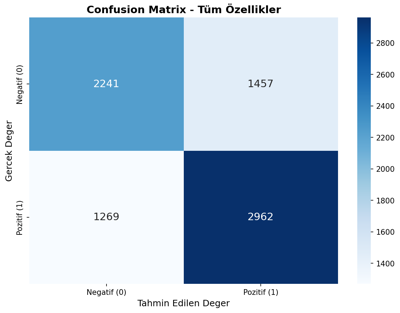
\includegraphics{confusion_matrix.png}
\caption{Karisiklik Matrisi}
\label{fig:confusion}
\end{figure}

\begin{figure}[H]
\centering
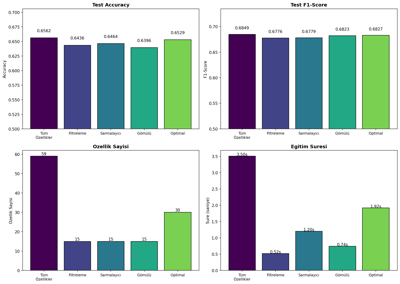
\includegraphics{results_comparison.png}
\caption{Yontem Karsilastirmasi}
\label{fig:comparison}
\end{figure}

% ============================================================================
% TARTIŞMA
% ============================================================================
\section{Tartışma}

\subsection{Araştırma Sorularının Yanıtlanması}

\textbf{AS1: Özellik seçimi yöntemleri sınıflandırma performansını nasıl etkiler?}

Deneysel sonuçlar, özellik seçiminin performansta \%1-2 oranında kabul edilebilir bir düşüşe neden olduğunu göstermiştir. 59 özellikten 15'e inildiğinde (\%75 azalma) performans yalnızca \%1-2 düşmüştür. Bu sonuç, veri kümesindeki birçok özelliğin gereksiz (redundant) veya gürültülü (noisy) olduğunu göstermektedir.

\textbf{AS2: Hangi özellik seçimi yöntemi en iyi performans-verimlilik dengesini sağlar?}

\begin{itemize}
    \item \textbf{Performans açısından:} Sarmalayıcı (RFE) en iyi sonucu (\%64.64) üretmiştir.
    \item \textbf{Verimlilik açısından:} Filtreleme yöntemi en hızlı eğitim süresine (0.52s) sahiptir.
    \item \textbf{Denge açısından:} Gömülü yöntem makul performans (0.6396) ve makul süre (0.74s) ile iyi bir denge sunmaktadır.
\end{itemize}

Uygulama gereksinimlerine göre:
\begin{itemize}
    \item Maksimum performans gerekiyorsa: RFE tercih edilmelidir.
    \item Hız kritikse: Filtreleme yöntemi tercih edilmelidir.
    \item Dengeli yaklaşım gerekiyorsa: Gömülü yöntem tercih edilmelidir.
\end{itemize}

\textbf{AS3: Ortak seçilen özelliklerin yorumu nedir?}

Beş ortak özelliğin analizi, haber popülerliğini etkileyen üç ana faktörü ortaya koymuştur:

\begin{enumerate}
    \item \textbf{Anahtar Kelime Stratejisi:} kw\_avg\_avg ve kw\_min\_avg özellikleri, SEO ve içerik pazarlamasının önemini göstermektedir.
    
    \item \textbf{Yayın Zamanlaması:} is\_weekend özelliği, kullanıcı davranışlarının zamana bağlı değişkenliğini yansıtmaktadır.
    
    \item \textbf{Konu İçeriği:} LDA\_01 ve LDA\_02 özellikleri, haberin konu alanının popülerlik üzerindeki etkisini göstermektedir.
\end{enumerate}

\textbf{AS4: Optimum özellik sayısı kaçtır?}

Optimum özellik sayısı 30 olarak belirlenmiştir. Bu sayı ile:
\begin{itemize}
    \item CV Accuracy: \%65.20 (59 özellik ile \%65.25)
    \item Test Accuracy: \%65.29 (59 özellik ile \%65.62)
    \item Özellik azaltma: \%49
    \item Süre azaltma: \%45
\end{itemize}

30 özellik, performans kaybını minimize ederken hesaplama verimliliğini artırmaktadır.

\subsection{Sınırlılıklar ve Gelecek Çalışmalar}

Bu çalışmanın bazı sınırlılıkları bulunmaktadır:

\begin{enumerate}
    \item \textbf{Model Çeşitliliği:} Yalnızca Lojistik Regresyon kullanılmıştır. Farklı sınıflandırıcılar (SVM, Neural Networks) ile karşılaştırma yapılabilir.
    
    \item \textbf{Özellik Etkileşimleri:} Özellikler arası etkileşimler değerlendirilmemiştir. Polynomial features veya neural networks bu etkileşimleri yakalayabilir.
    
    \item \textbf{Zamansal Faktörler:} Veri kümesindeki zamansal trendler detaylı analiz edilmemiştir.
\end{enumerate}

Gelecek çalışmalarda:
\begin{itemize}
    \item Ensemble yöntemler ile özellik seçimi kombinasyonları denenebilir.
    \item Deep learning modelleri ile otomatik özellik öğrenimi karşılaştırılabilir.
    \item Transfer learning yaklaşımları değerlendirilebilir.
\end{itemize}

% ============================================================================
% SONUÇ
% ============================================================================
\section{Sonuç}

Bu çalışmada, Online News Popularity veri kümesi üzerinde üç farklı özellik seçimi paradigması (Filtreleme, Sarmalayıcı ve Gömülü) sistematik olarak karşılaştırılmıştır. Elde edilen bulgular şu şekilde özetlenebilir:

\begin{enumerate}
    \item \textbf{Performans:} Tüm özelliklerin kullanıldığı durumda \%65.62 test doğruluğu elde edilmiştir. Özellik seçimi yöntemleri, 15 özellik ile \%64-65 arasında benzer performans sergilemiştir.
    
    \item \textbf{Verimlilik:} Özellik seçimi, eğitim süresini \%66-85 oranında azaltmıştır.
    
    \item \textbf{En İyi Yöntem:} Sarmalayıcı (RFE) yöntemi, performans açısından en iyi sonucu (\%64.64) üretmiştir.
    
    \item \textbf{Optimum Özellik Sayısı:} 30 özellik ile \%65.29 doğruluk elde edilmiş, performans-verimlilik dengesi sağlanmıştır.
    
    \item \textbf{Kritik Özellikler:} Anahtar kelime metrikleri, yayın zamanlaması ve LDA konu skorları, haber popülerliği için en ayırt edici faktörler olarak belirlenmiştir.
\end{enumerate}

Sonuç olarak, özellik seçimi makine öğrenmesi projelerinde model yorumlanabilirliğini artırırken hesaplama maliyetini düşüren etkili bir stratejidir. Bu çalışma, farklı özellik seçimi yöntemlerinin güçlü ve zayıf yönlerini ortaya koyarak uygulayıcılara yol gösterici bilgiler sunmaktadır.

% ============================================================================
% KAYNAKLAR
% ============================================================================
\begin{thebibliography}{99}

\bibitem{guyon2003introduction}
I. Guyon and A. Elisseeff, ``An introduction to variable and feature selection,'' \textit{Journal of Machine Learning Research}, vol. 3, pp. 1157--1182, 2003.

\bibitem{chandrashekar2014survey}
G. Chandrashekar and F. Sahin, ``A survey on feature selection methods,'' \textit{Computers \& Electrical Engineering}, vol. 40, no. 1, pp. 16--28, 2014.

\bibitem{fernandes2015proactive}
K. Fernandes, P. Vinagre, and P. Cortez, ``A proactive intelligent decision support system for predicting the popularity of online news,'' in \textit{Proceedings of the 17th Portuguese Conference on Artificial Intelligence (EPIA)}, 2015, pp. 535--546.

\bibitem{guyon2002gene}
I. Guyon, J. Weston, S. Barnhill, and V. Vapnik, ``Gene selection for cancer classification using support vector machines,'' \textit{Machine Learning}, vol. 46, no. 1-3, pp. 389--422, 2002.

\bibitem{breiman2001random}
L. Breiman, ``Random forests,'' \textit{Machine Learning}, vol. 45, no. 1, pp. 5--32, 2001.

\bibitem{pedregosa2011scikit}
F. Pedregosa, G. Varoquaux, A. Gramfort, et al., ``Scikit-learn: Machine learning in Python,'' \textit{Journal of Machine Learning Research}, vol. 12, pp. 2825--2830, 2011.

\bibitem{kohavi1997wrappers}
R. Kohavi and G. H. John, ``Wrappers for feature subset selection,'' \textit{Artificial Intelligence}, vol. 97, no. 1-2, pp. 273--324, 1997.

\bibitem{liu1998feature}
H. Liu and H. Motoda, \textit{Feature Extraction, Construction and Selection: A Data Mining Perspective}. Springer, 1998.

\end{thebibliography}

\end{document}
